\documentclass[tikz,border=2pt]{standalone}

\usepackage{palatino}
\usetikzlibrary{positioning}

\definecolor{queryBg}{HTML}{EBF3FE}
\definecolor{replyBg}{HTML}{F4F4F5}
\definecolor{queryText}{HTML}{1E3A8A}
\definecolor{replyText}{HTML}{27272A}

\newlength{\figurewidth}
\setlength{\figurewidth}{16cm}

\begin{document}
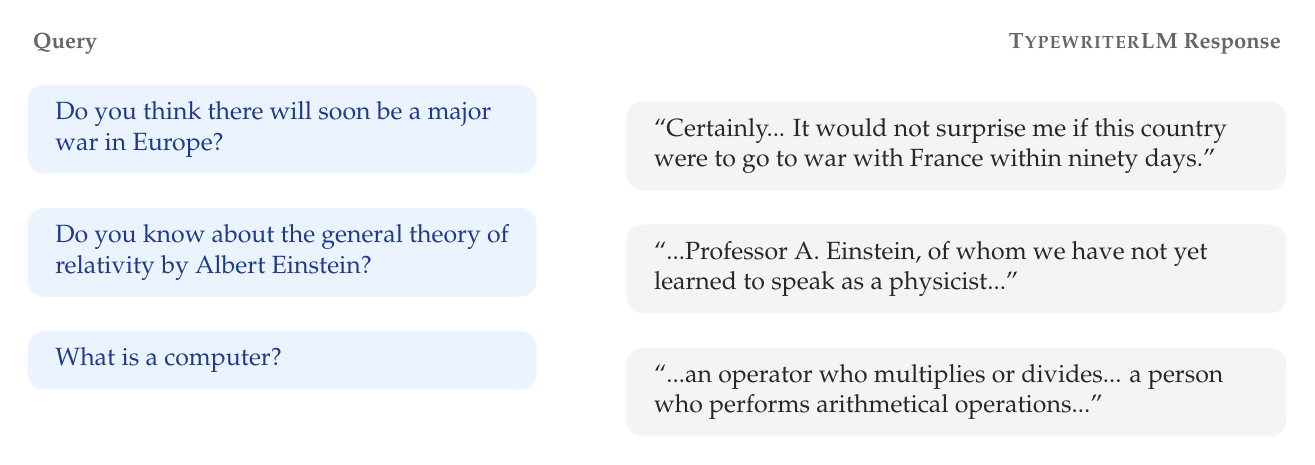
\begin{tikzpicture}[
    node distance=0.3cm,
    bubble/.style={
        rounded corners=6pt,
        inner xsep=10pt,
        inner ysep=6pt,
        align=flush left,
        font=\small\linespread{1.0}\selectfont
    },
    query/.style={
        bubble,
        text width=0.36\figurewidth,
        fill=queryBg,
        text=queryText
    },
    reply/.style={
        bubble,
        text width=0.48\figurewidth,
        fill=replyBg,
        text=replyText
    },
    header/.style={
        font=\footnotesize\bfseries,
        text=gray!80!black,
        inner sep=2pt
    }
]
    \node[header] (qHead) at (0,0) [anchor=west] {Query};
    \node[header] (rHead) at (\figurewidth,0) [anchor=east]
        {\textsc{TypewriterLM} Response};

    \node[query,below=of qHead.south west,anchor=north west] (q1) {
        Do you think there will soon be a major war in Europe?
    };
    \node[reply,yshift=-6pt] (r1) at (q1.north -| rHead.east)
        [anchor=north east] {
        ``Certainly... It would not surprise me if this country were to go
        to war with France within ninety days.''
    };

    \node[query,below=12pt of q1.south west,anchor=north west] (q2) {
        Do you know about the general theory of relativity by Albert Einstein?
    };
    \node[reply,yshift=-6pt] (r2) at (q2.north -| r1.north east)
        [anchor=north east] {
        ``...Professor A. Einstein, of whom we have not yet learned to speak
        as a physicist...''
    };

    \node[query,below=12pt of q2.south west,anchor=north west] (q3) {
        What is a computer?
    };
    \node[reply,yshift=-6pt] (r3) at (q3.north -| r2.north east)
        [anchor=north east] {
        ``...an operator who multiplies or divides... a person who performs
        arithmetical operations...''
    };
\end{tikzpicture}
\end{document}
